\documentclass[compress]{beamer}
\mode<presentation>
{
 \usetheme{Vilanova}
}

\usepackage[english]{babel}

\usepackage[latin1]{inputenc}

\usepackage{times}
\usepackage[T1]{fontenc}

\usepackage{amsfonts}
\usepackage{amsmath}
\usepackage{amssymb}
\usepackage{tikz}
%\usepackage{url}
\usepackage[normal]{subfigure}
\newcommand{\goodgap}{%
	\hspace{\subfigtopskip}%
	\hspace{\subfigbottomskip}}



%\newtheorem{definition}{Definition}

\title{ORFEO Tools for Map Updating}

\subtitle{OTB-Applications ``best of''} % (optional)

\author
{Jordi Inglada}
\normalsize

\institute[Cnes] % (optional, but mostly needed)
{\textsc{Centre national d'\'etudes spatiales}}

\date{}

\subject{New challenges}


\pgfdeclareimage[height=96mm,width=128mm]{background}{fondsClairSansLogo}
\setbeamertemplate{background}{\pgfuseimage{background}}
\pgfdeclareimage[height=0.6cm]{logoIncrust}{logoIncrust}
\pgfdeclareimage[height=0.6cm]{logo_cnes}{logo_cnes}
\logo{
\begin{tabular}{lp{0.14\textwidth}lp{0.25\textwidth}r}
\href{http://www.cnes.fr}{\pgfuseimage{logo_cnes}}
&&\footnotesize{ARMURS Workshop, Brussels, 2008/09/25}&&
\href{http://www.orfeo-toolbox.org}{\pgfuseimage{logoIncrust}}\\
\end{tabular}
}



% Delete this, if you do not want the table of contents to pop up at
% the beginning of each subsection:
\AtBeginSubsection[]
{
  \begin{frame}<beamer>
    \frametitle{Outline}
    \tableofcontents[currentsection,currentsubsection]
  \end{frame}
}




% If you wish to uncover everything in a step-wise fashion, uncomment
% the following command: 

\beamerdefaultoverlayspecification{<+->}

\begin{document}

\begin{frame}
  \titlepage
\end{frame}

%\section*{Introduction}
\begin{frame}
    \frametitle{Introduction}
  \begin{itemize}
    \item New HR/VHR sensors and systems are becoming available
    \item Spatial, spectral and temporal resolution have very much
    increased in the last few years
  \item Many operational sensors allow multi-sensor synergy
    \item Other sources of geographical information: maps, GIS,
    GoogleEarth, ...
  \item End users are becoming aware of all these possibilities and
  ask for operational tools to deal with large amounts of data in an
  efficient way
  \end{itemize}
\end{frame}

\begin{frame}
\frametitle{Scope}
\begin{itemize}
  \item ORFEO Preparatory Program
    \item Pleiades + Cosmo Skymed
    \item Thematic Part
      \begin{itemize}
	\item Users' needs (extracted information)
	\item Product definition
	\item Validation
      \end{itemize}
    \item Methodological Part
    \begin{itemize}
    \item Coordination of research activities in Image Processing
    \item ORFEO Toolbox, OTB,~ ~\url{http://www.orfeo-toolbox.org}
    \end{itemize}
    \item What is needed / What is feasible
    \item Automatic and semi-automatic approaches for
      \begin{itemize}
      \item image classification and segmentation, change detection, etc.
      \end{itemize}
 \end{itemize}
\end{frame}

%% \begin{frame}
%%     \frametitle{Introduction}
%%   \begin{itemize}
%%     \item In the frame of the ORFEO Preparatory Program
%%     \item Map updating across applications
%%       \begin{itemize}
%% 	\item Thematic groups
%%       \end{itemize}
%%     \item Automatic and semi-automatic approaches for
%%       \begin{itemize}
%% 	\item image classification and segmentation, change detection, etc.
%%       \end{itemize}
%%     \item OTB-Applications
%%   \end{itemize}
%% \end{frame}

\section{Map updating}
\begin{frame}
  \frametitle{Map updating}
  \framesubtitle{Main steps}
  \begin{enumerate}
    \item Ortho-rectification and fine registration
    \item Pan-sharpening
    \item Feature extraction
    \item Image classification
    \item Change detection
    \item Object segmentation
  \end{enumerate}
\end{frame}


\section{OTB Applications}
\subsection{Ortho-rectification}

\begin{frame}
  \frametitle{Ortho-rectification}
      \begin{center}
      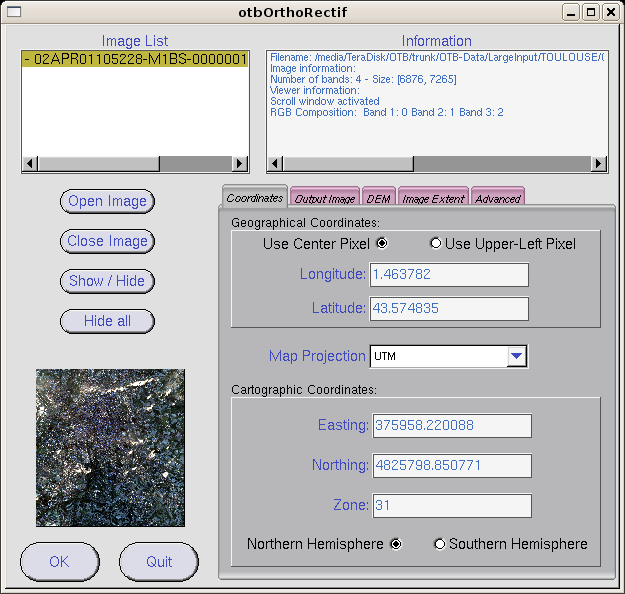
\includegraphics[width=0.80\textwidth]{Images/ortho1.png}
  \end{center}
\end{frame}

\begin{frame}
  \frametitle{Ortho-rectification}
      \begin{center}
      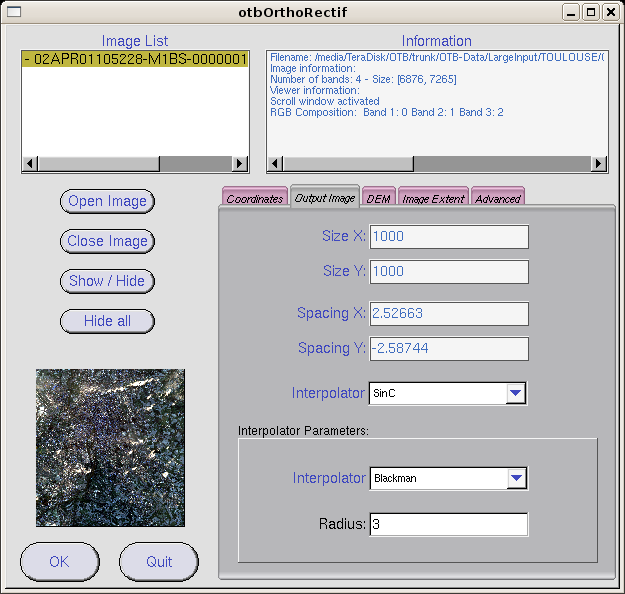
\includegraphics[width=0.80\textwidth]{Images/ortho2.png}
  \end{center}
\end{frame}

\begin{frame}
  \frametitle{Ortho-rectification}
      \begin{center}
      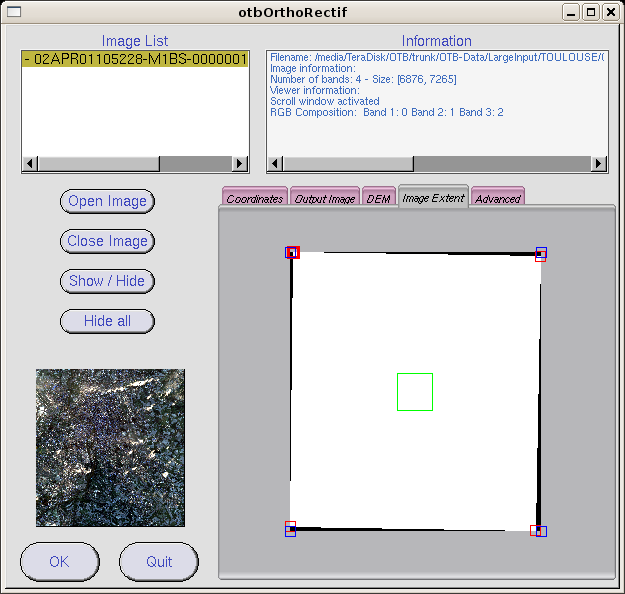
\includegraphics[width=0.80\textwidth]{Images/ortho3.png}
  \end{center}
\end{frame}



\subsection{Pan-sharpening}

\begin{frame}
  \frametitle{Pan-sharpening}
      \begin{center}
      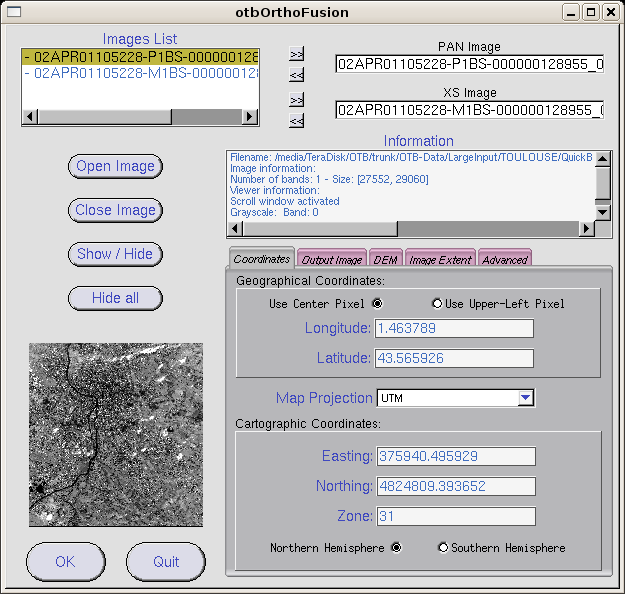
\includegraphics[width=0.80\textwidth]{Images/pansharp.png}
  \end{center}
\end{frame}


\subsection{Feature extraction}

\begin{frame}
  \frametitle{Feature Extraction}
      \begin{center}
      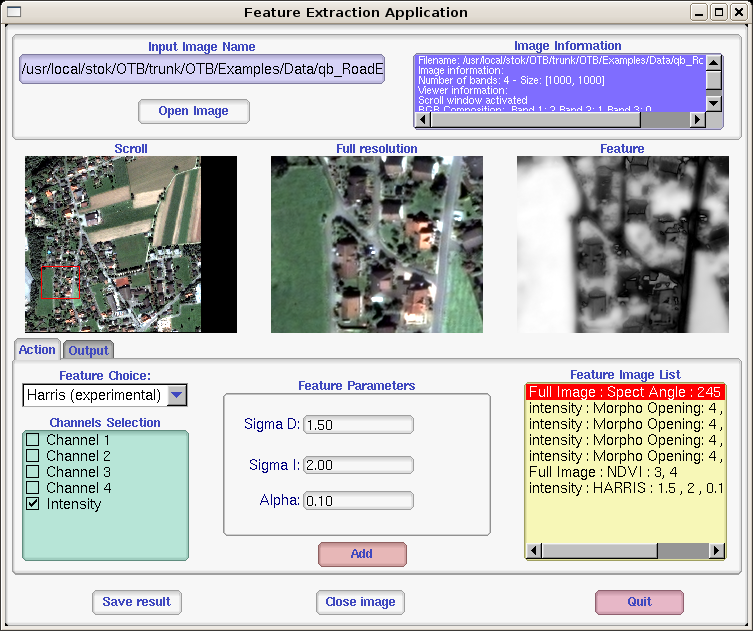
\includegraphics[width=0.80\textwidth]{Images/feature1.png}
  \end{center}
\end{frame}


\begin{frame}
  \frametitle{Feature Extraction}
      \begin{center}
      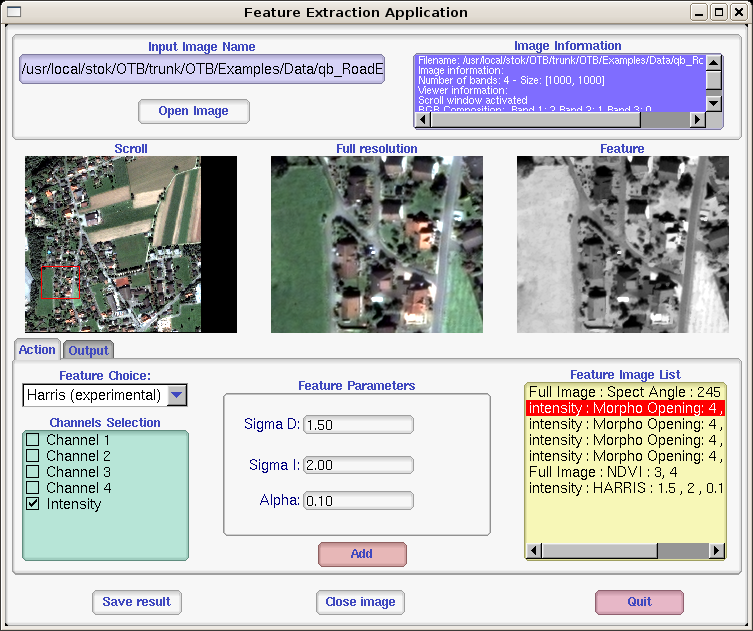
\includegraphics[width=0.80\textwidth]{Images/feature2.png}
  \end{center}
\end{frame}


\begin{frame}
  \frametitle{Feature Extraction}
      \begin{center}
      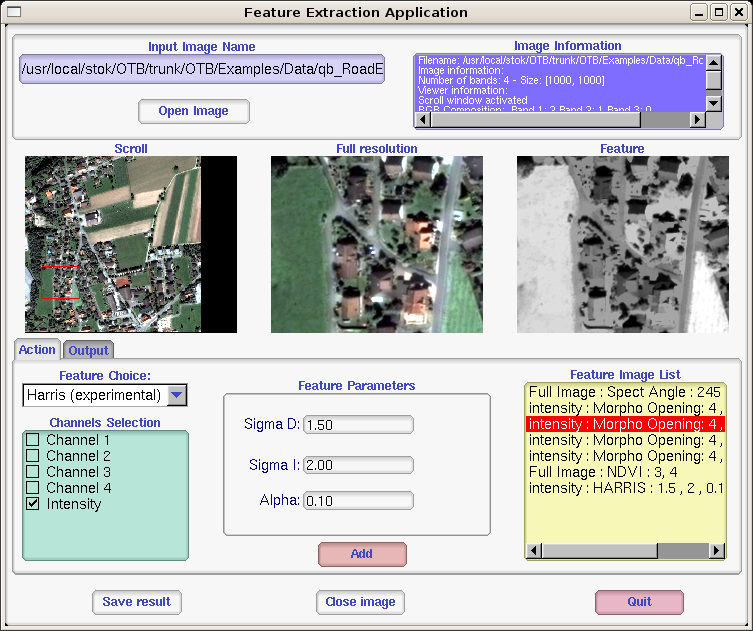
\includegraphics[width=0.80\textwidth]{Images/feature3.png}
  \end{center}
\end{frame}


\begin{frame}
  \frametitle{Feature Extraction}
      \begin{center}
      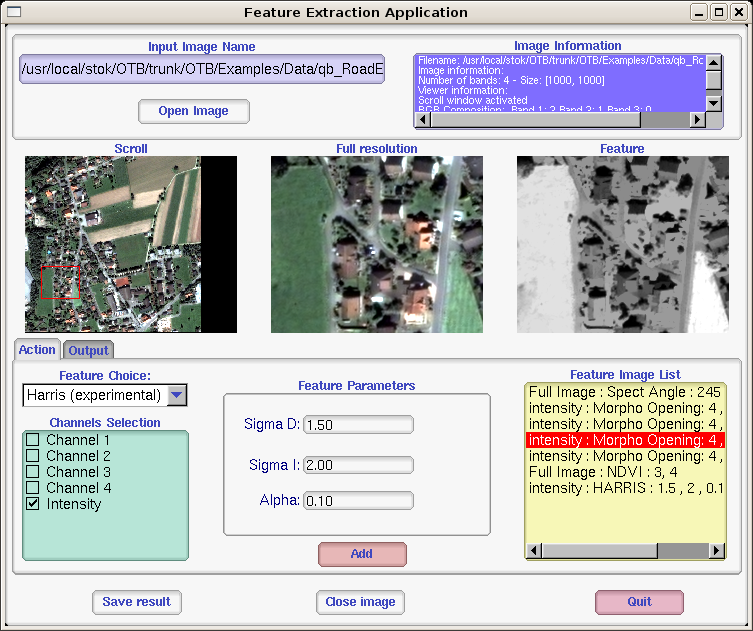
\includegraphics[width=0.80\textwidth]{Images/feature4.png}
  \end{center}
\end{frame}


\begin{frame}
  \frametitle{Feature Extraction}
      \begin{center}
      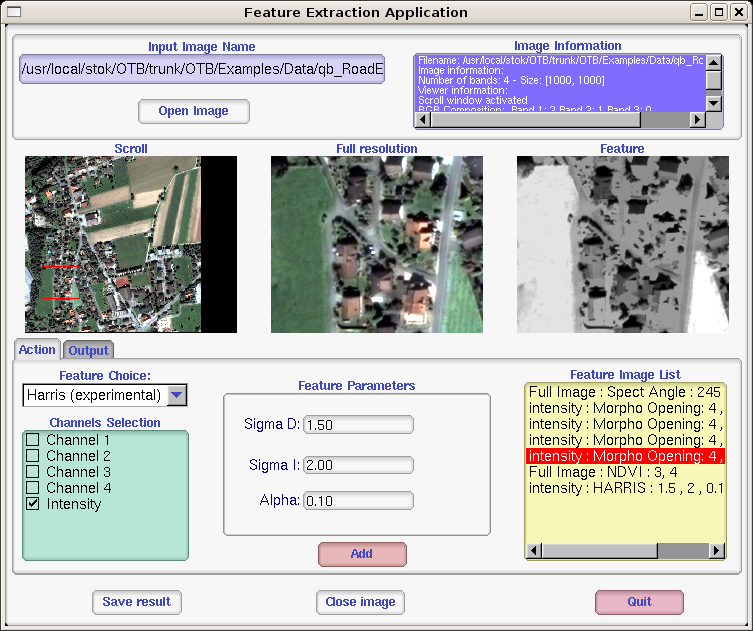
\includegraphics[width=0.80\textwidth]{Images/feature5.png}
  \end{center}
\end{frame}


\begin{frame}
  \frametitle{Feature Extraction}
      \begin{center}
      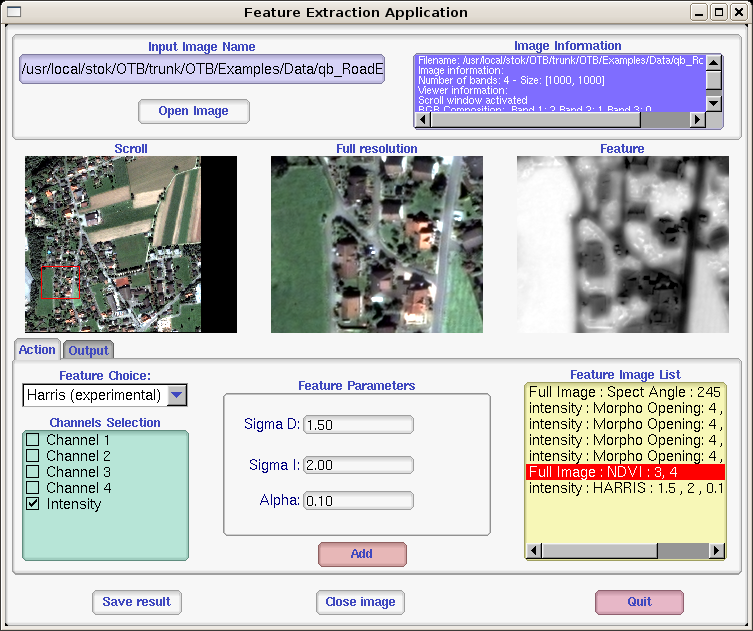
\includegraphics[width=0.80\textwidth]{Images/feature6.png}
  \end{center}
\end{frame}


\begin{frame}
  \frametitle{Feature Extraction}
      \begin{center}
      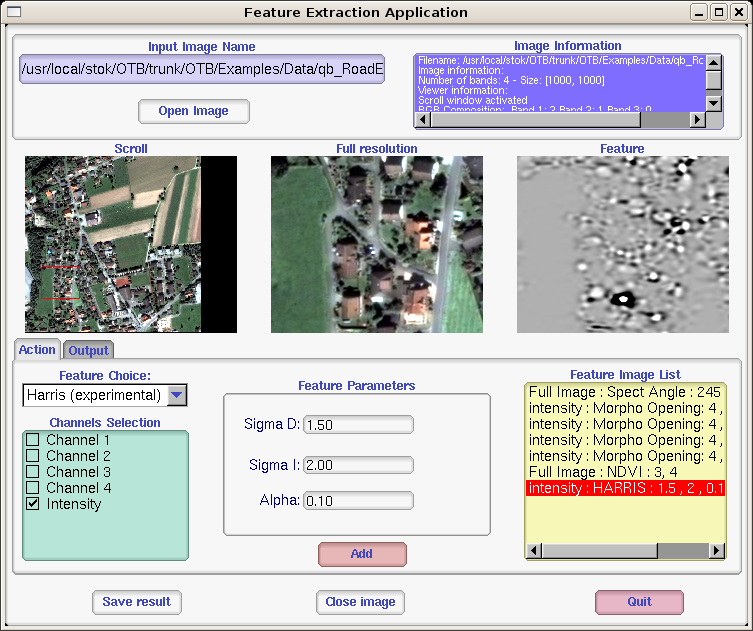
\includegraphics[width=0.80\textwidth]{Images/feature7.png}
  \end{center}
\end{frame}

\begin{frame}
  \frametitle{Feature Extraction}
      \begin{center}
      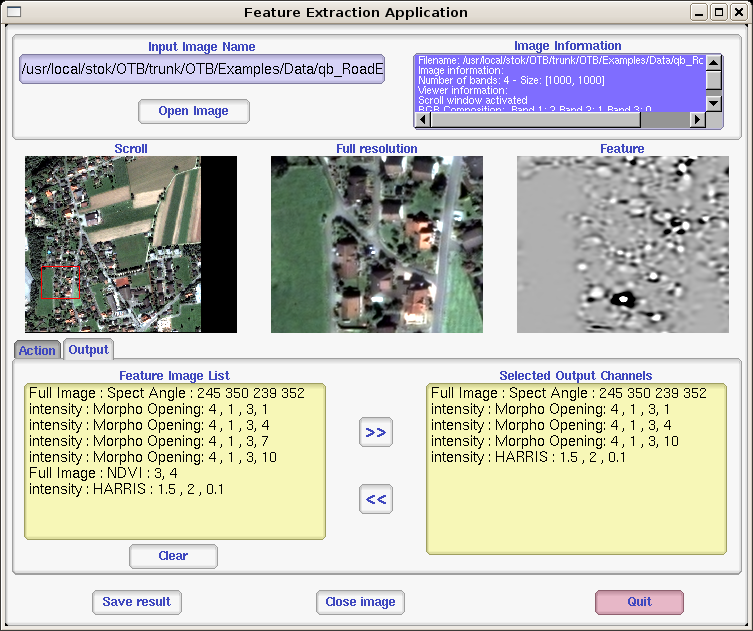
\includegraphics[width=0.80\textwidth]{Images/feature8.png}
  \end{center}
\end{frame}



\subsection{Image classification}

\begin{frame}
  \frametitle{Supervised image classification}
      \begin{center}
      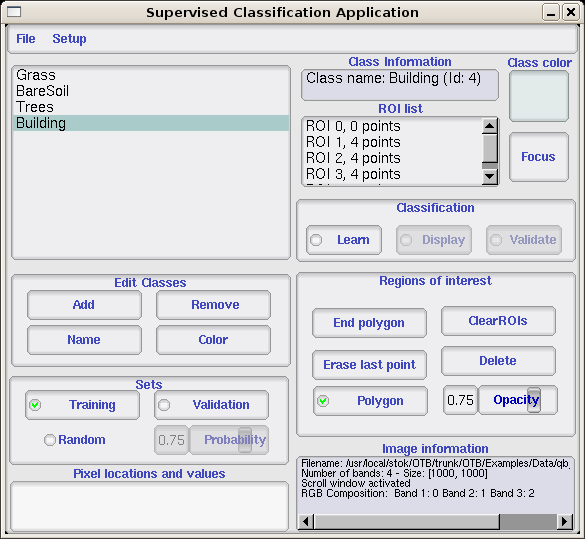
\includegraphics[width=0.85\textwidth]{Images/classifGUI.png}
  \end{center}
\end{frame}

\begin{frame}
  \frametitle{Supervised image classification}
      \begin{center}
      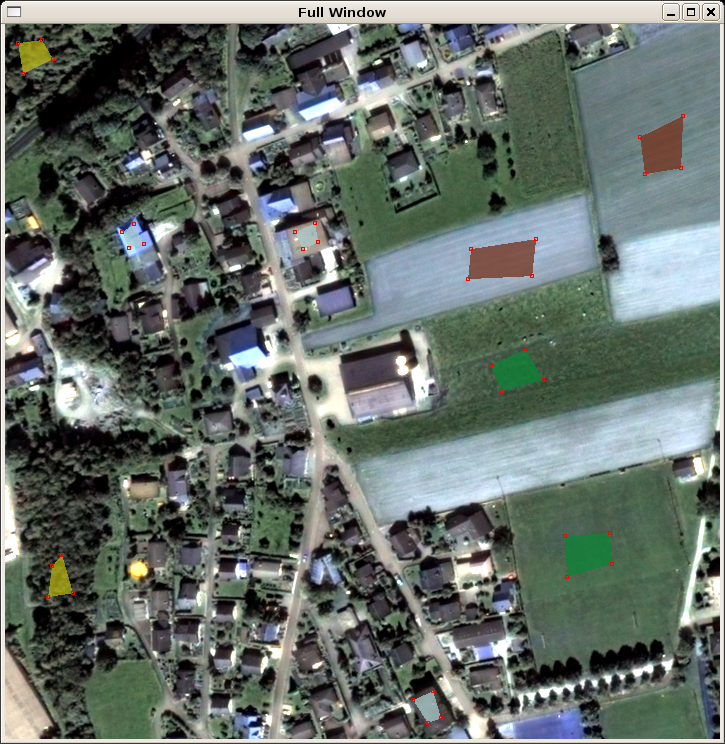
\includegraphics[width=0.85\textwidth]{Images/classfTrain.png}
  \end{center}
\end{frame}

\begin{frame}
  \frametitle{Supervised image classification}
      \begin{center}
      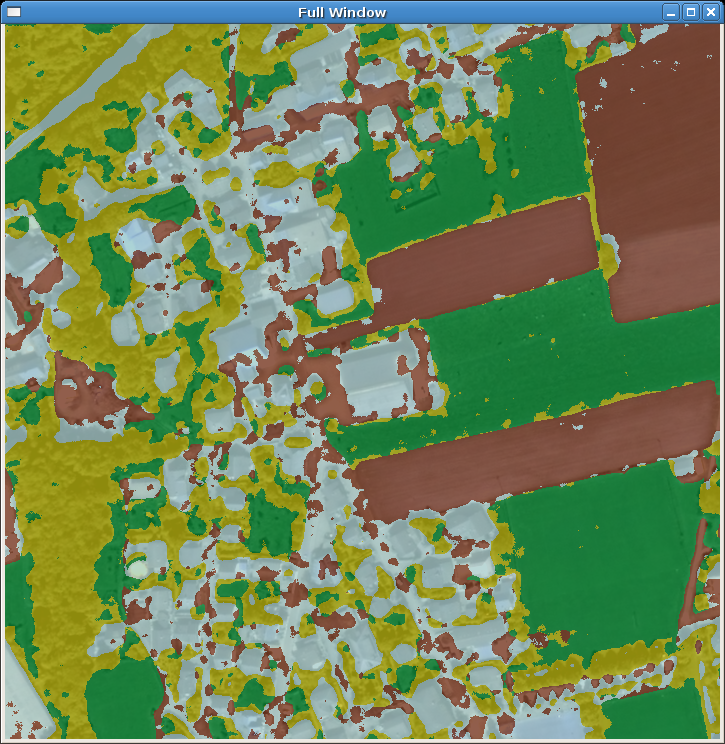
\includegraphics[width=0.85\textwidth]{Images/classfResult.png}
  \end{center}
\end{frame}

\begin{frame}
  \frametitle{Supervised image classification}
      \begin{center}
      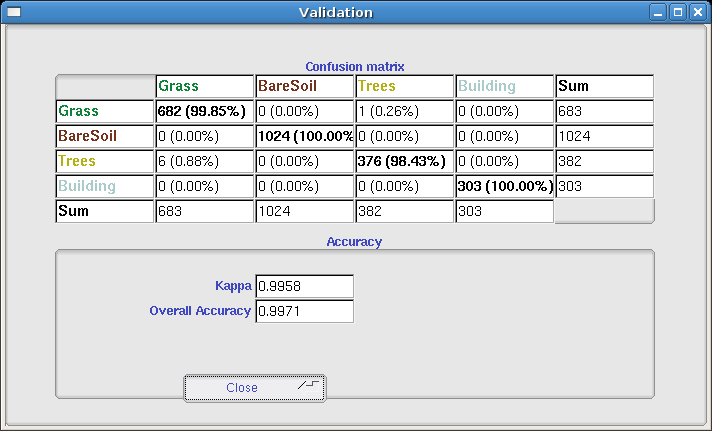
\includegraphics[width=0.85\textwidth]{Images/classfValid.png}
  \end{center}
\end{frame}


\subsection{Change detection}
\begin{frame}
  \frametitle{Supervised change detection}
      \begin{center}
      \includegraphics[width=0.85\textwidth]{../SummerSchool2008/TalkMonday/Images/icd.png}
  \end{center}
\end{frame}

\subsection{Object segmentation}

\begin{frame}
  \frametitle{Object segmentation}
      \begin{center}
      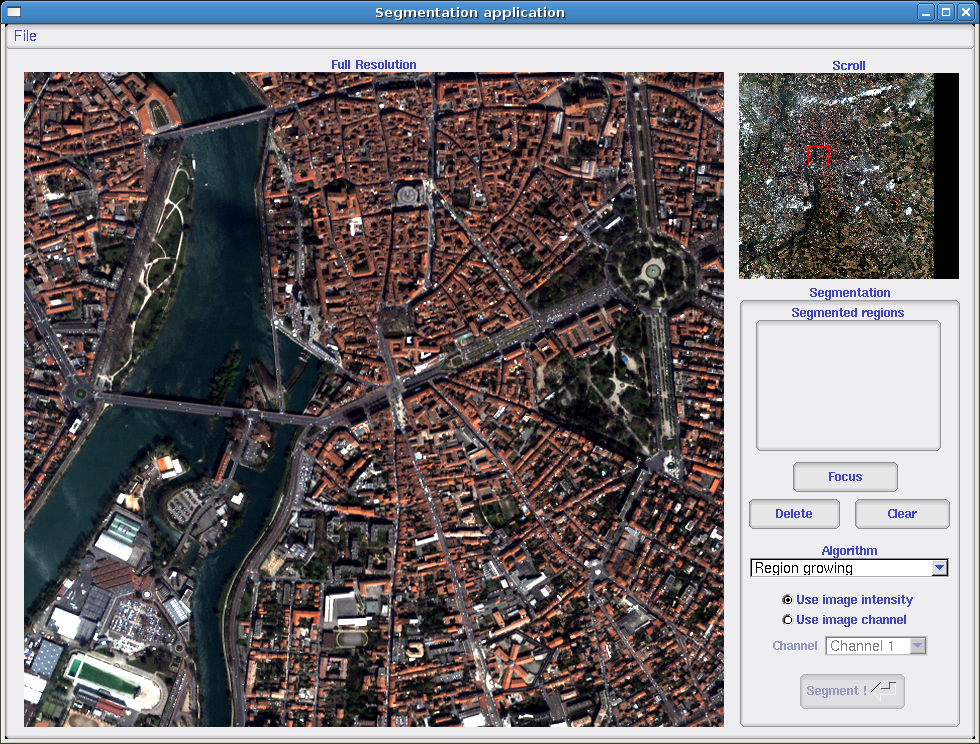
\includegraphics[width=0.80\textwidth]{Images/seg1.png}
  \end{center}
\end{frame}

\begin{frame}
  \frametitle{Object segmentation}
      \begin{center}
      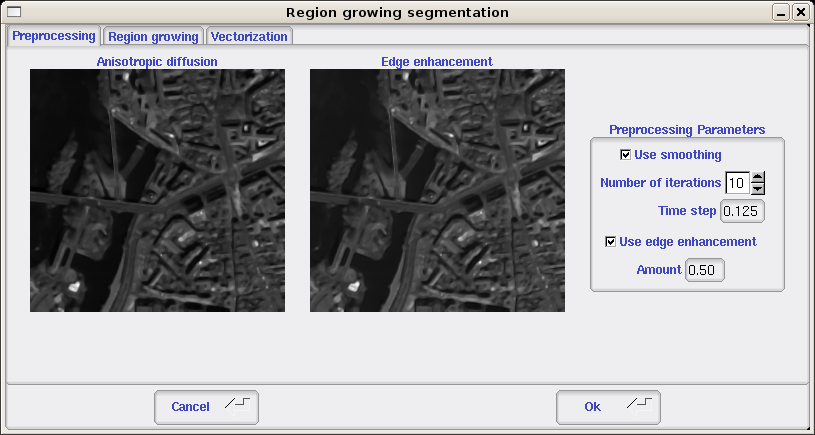
\includegraphics[width=0.80\textwidth]{Images/seg2.png}
  \end{center}
\end{frame}

\begin{frame}
  \frametitle{Object segmentation}
      \begin{center}
      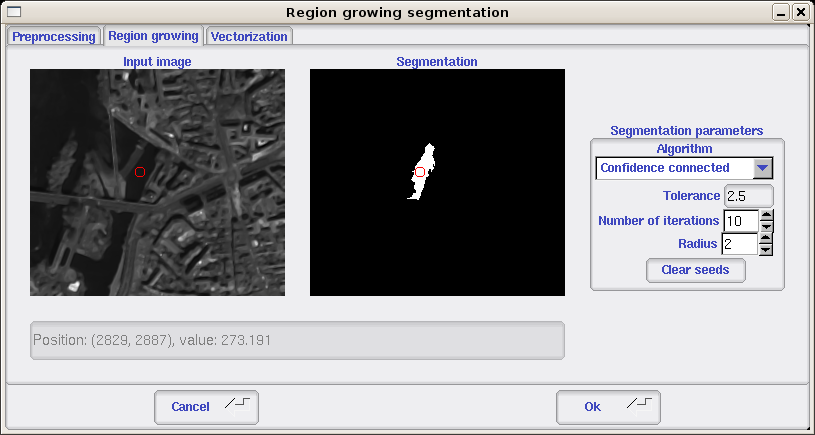
\includegraphics[width=0.80\textwidth]{Images/seg3.png}
  \end{center}
\end{frame}

\begin{frame}
  \frametitle{Object segmentation}
      \begin{center}
      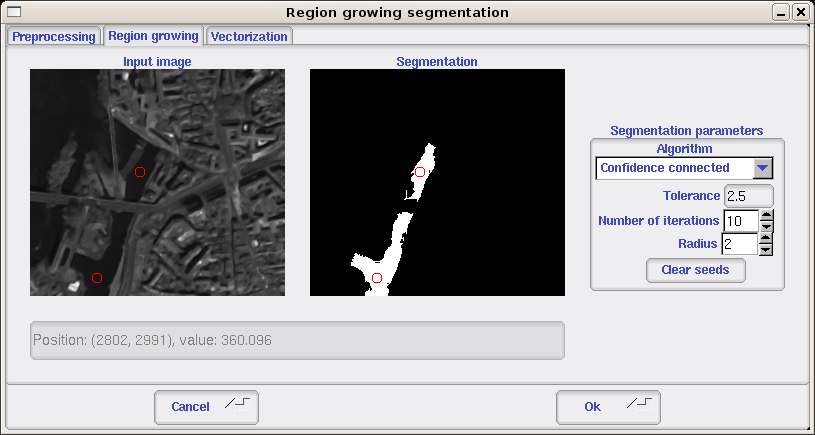
\includegraphics[width=0.80\textwidth]{Images/seg4.png}
  \end{center}
\end{frame}

\begin{frame}
  \frametitle{Object segmentation}
      \begin{center}
      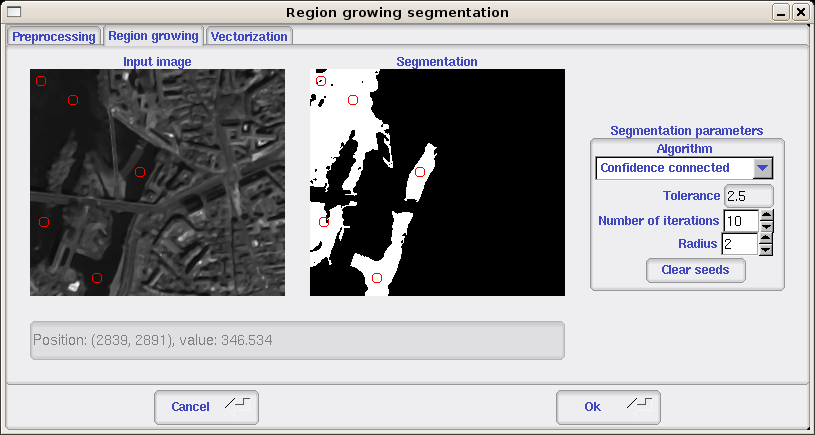
\includegraphics[width=0.80\textwidth]{Images/seg5.png}
  \end{center}
\end{frame}

\begin{frame}
  \frametitle{Object segmentation}
      \begin{center}
      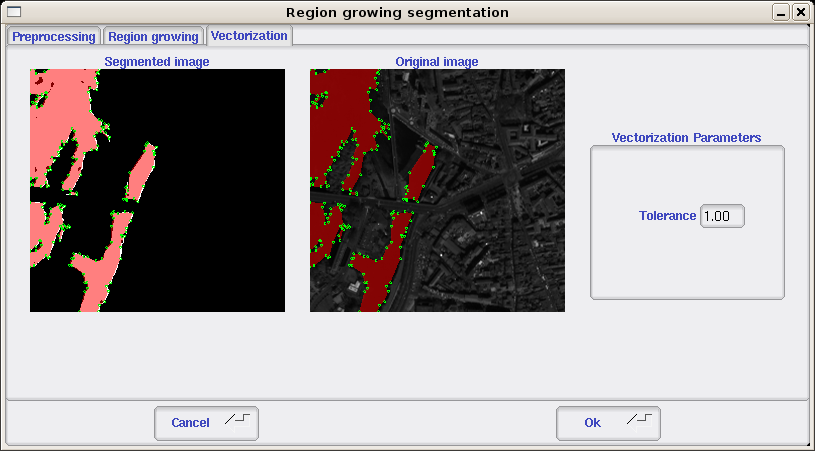
\includegraphics[width=0.80\textwidth]{Images/seg6.png}
  \end{center}
\end{frame}

\begin{frame}
  \frametitle{Object segmentation}
      \begin{center}
      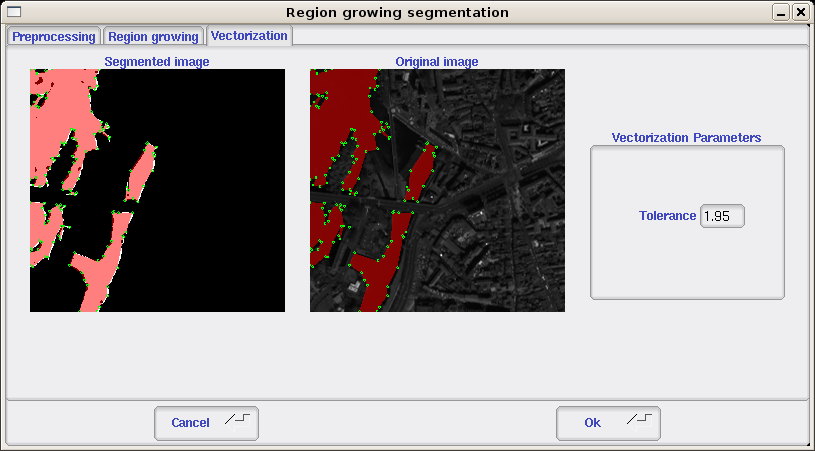
\includegraphics[width=0.80\textwidth]{Images/seg7.png}
  \end{center}
\end{frame}

\begin{frame}
  \frametitle{Object segmentation}
      \begin{center}
      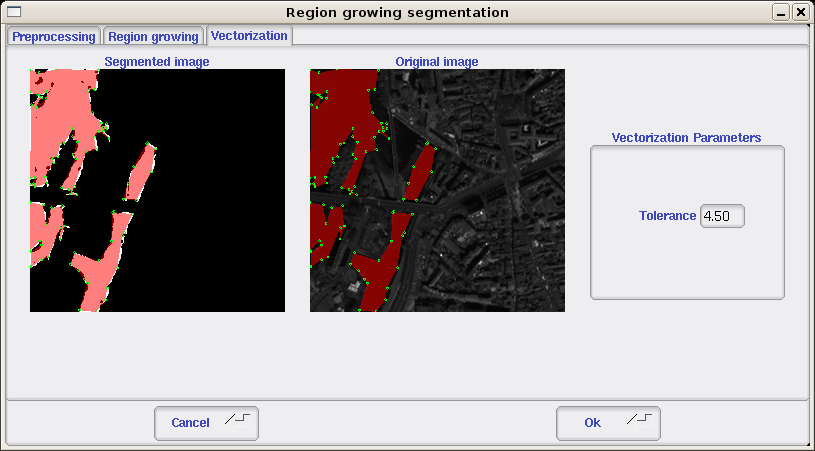
\includegraphics[width=0.80\textwidth]{Images/seg8.png}
  \end{center}
\end{frame}

\begin{frame}
  \frametitle{Object segmentation}
      \begin{center}
      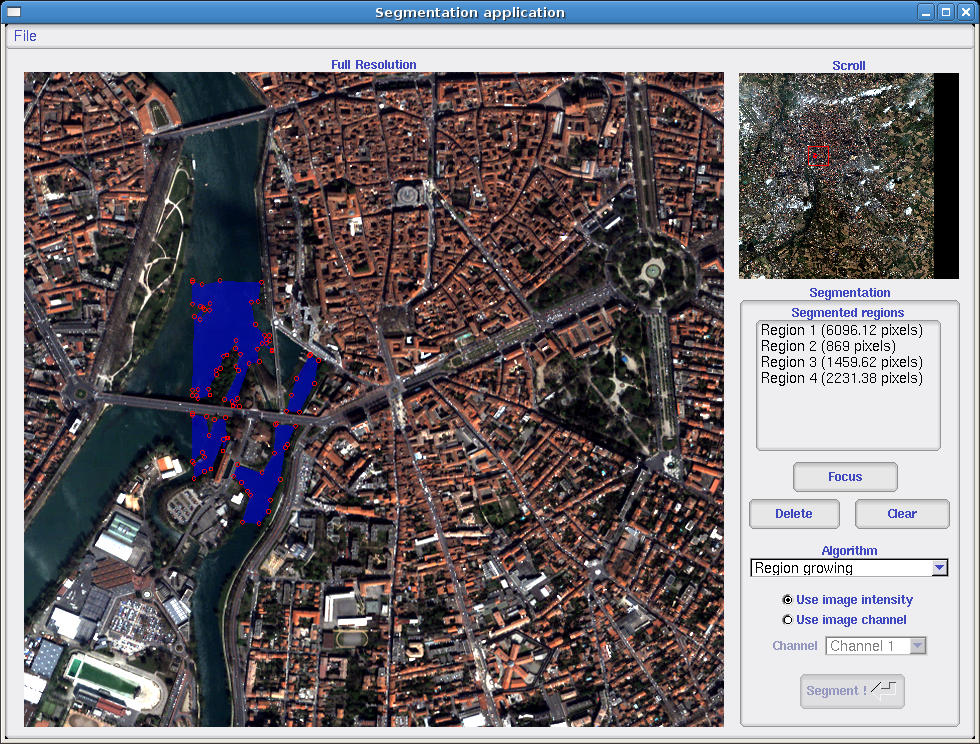
\includegraphics[width=0.80\textwidth]{Images/seg9.png}
  \end{center}
\end{frame}

\begin{frame}
  \frametitle{Object segmentation}
      \begin{center}
      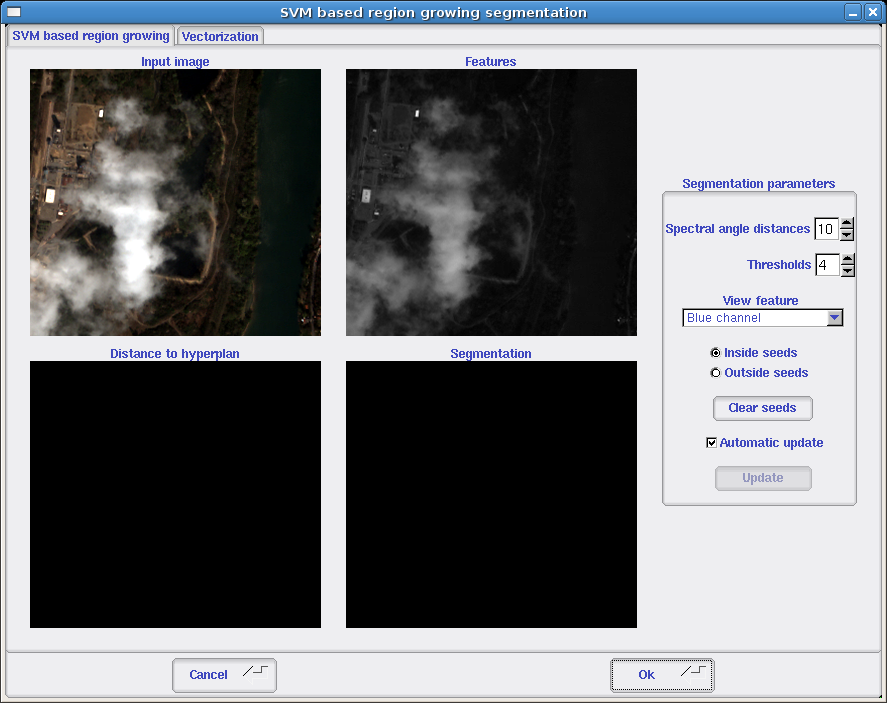
\includegraphics[width=0.80\textwidth]{Images/seg10.png}
  \end{center}
\end{frame}

\begin{frame}
  \frametitle{Object segmentation}
      \begin{center}
      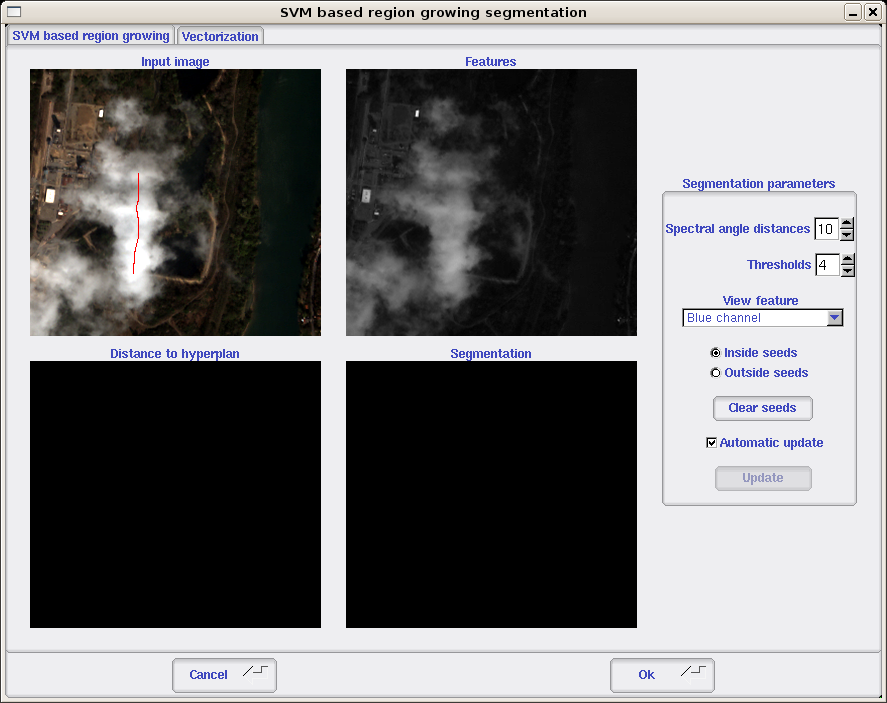
\includegraphics[width=0.80\textwidth]{Images/seg11.png}
  \end{center}
\end{frame}

\begin{frame}
  \frametitle{Object segmentation}
      \begin{center}
      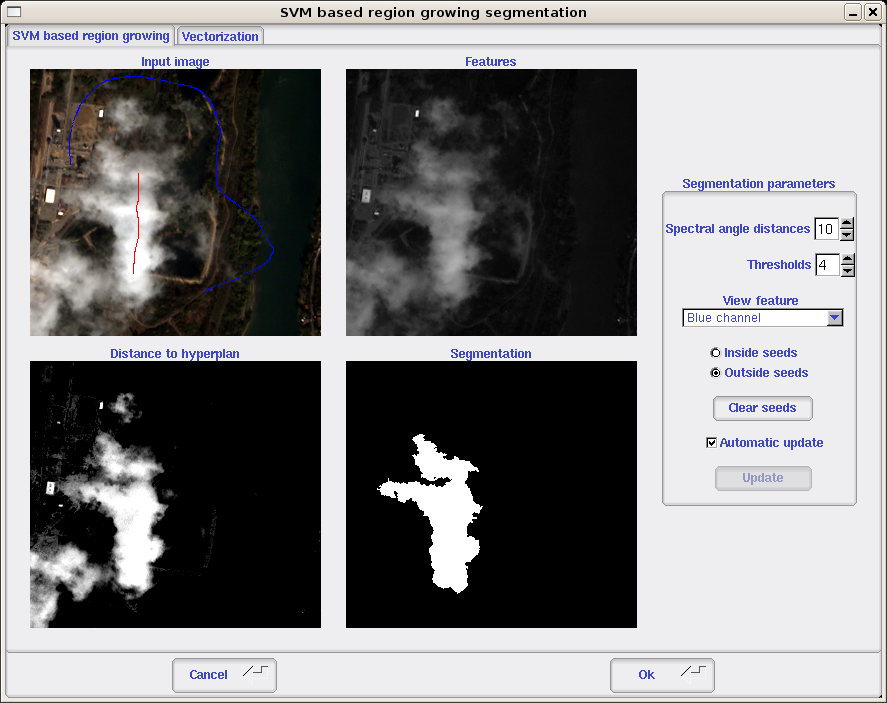
\includegraphics[width=0.80\textwidth]{Images/seg12.png}
  \end{center}
\end{frame}

\begin{frame}
  \frametitle{Object segmentation}
      \begin{center}
      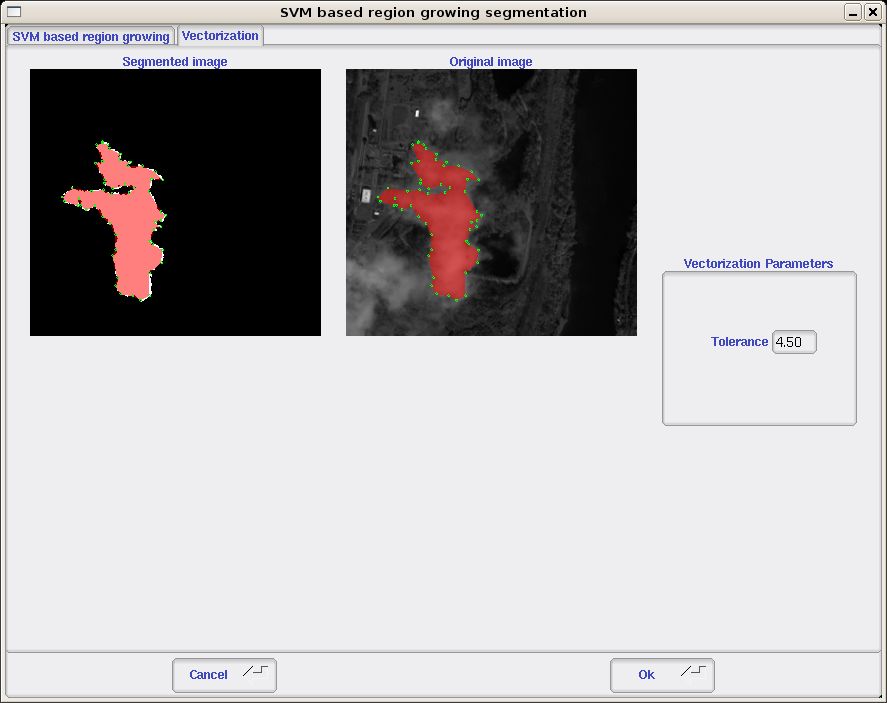
\includegraphics[width=0.80\textwidth]{Images/seg13.png}
  \end{center}
\end{frame}

\begin{frame}
  \frametitle{Object segmentation}
      \begin{center}
      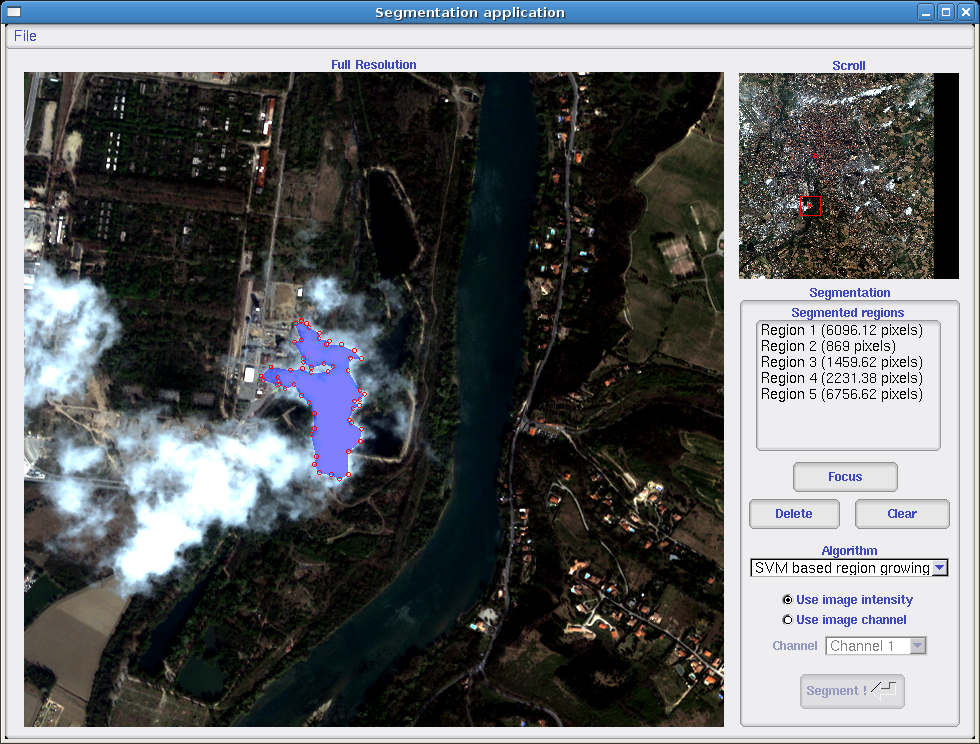
\includegraphics[width=0.80\textwidth]{Images/seg14.png}
  \end{center}
\end{frame}




\section{Conclusion}
\begin{frame}
  \frametitle{Conclusion}
  \begin{itemize}
    \item Map updating is made of several sequential steps
      \begin{itemize}
	\item From ortho-registration to object segmentation
      \end{itemize}
    \item Automatic and semi-automatic approaches are complementary
    \item Interest of the active learning approaches
    \item OTB-Applications: growing set of tools for image information
    extraction
  \end{itemize}
\end{frame}

\begin{frame}
  \frametitle{Coming soon}
  \begin{itemize}
    \item Image fine registration
    \item KML input/output: display and share on Google Earth
    \item Object counting
    \item Network extraction (roads, hydrography)
    \item Urban area extraction
    \item Image to data base registration
  \end{itemize}
\end{frame}



%% \section[Data]{New data available}
%% \subsection[Spatial]{Spatial resolution}
%% \begin{frame}
%%   \frametitle{Spatial resolution}
%%   \begin{itemize}
%%     \item Increasing resolution in recent years:
%%       \begin{itemize}
%% 	\item Ikonos, Quickbird, Pleiades, Geoeye, etc.
%% 	\item Radarsat 2, Terra SAR X, COSMO Skymed, etc.
%%       \end{itemize}
%%     \item Metric resolution still needed:
%%       \begin{itemize}
%% 	\item The best choice for many applications: precision
%% 	farming, urban growing, some natural disasters, etc.
%% 	\item SPOT 5, Kompsat, Formosat, etc.
%%       \end{itemize}
%%     \item New decametric resolution systems will be launched:
%%       \begin{itemize}
%% 	\item Enough for some applications where the other 2
%% 	dimensions are more constrained.
%% 	\item ESA's Sentinel program
%%       \end{itemize}
%%   \end{itemize}
%% \end{frame}

%% \subsection[Spectral]{Spectral resolution}
%% \begin{frame}
%%   \frametitle{Spectral resolution}
%%   \begin{itemize}
%%     \item Most current optical systems are P+XS
%%       \begin{itemize}
%% 	\item 4 or 5 XS bands (B, G, R, NIR, SWIR)
%% 	\item often pan-sharpening is possible or even proposed as the
%% 	standard product
%%       \end{itemize}
%%     \item Not many space-borne hyper-spectral systems
%%     \item Raising interest for super-spectral systems
%%       \begin{itemize}
%% 	\item usually, a particular application only needs several
%% 	spectral bands
%% 	\item good balance between spatial and spectral resolutions
%% 	\item Sentinel-2, Ven$\mu$s
%%       \end{itemize}
%%       \item For SAR
%% 	\begin{itemize}
%% 	  \item Full polarimetry is expensive (in terms of power, thus
%% 	  resolution)
%% 	  \item Partial polarimetric systems (Envisat ASAR, COSMO
%% 	  Skymed)
%% 	  \begin{itemize}
%% 	    \item Raising interest for smart compact polarimetry concepts
%% 	  \end{itemize}
%% 	\end{itemize}
%%   \end{itemize}
%% \end{frame}

%% \subsection[Temporal]{Temporal resolution}
%% \begin{frame}
%%   \frametitle{Temporal resolution}
%%   \begin{itemize}
%%     \item Classical polar sun-synchronous orbits give revisit cycles
%%     of more than 20 days
%%     \item Revisit times are typically lowered by:
%%       \begin{itemize}
%% 	\item Changing viewing angles (affects radiometry)
%% 	\item Using more satellites (expensive)
%% 	\item Choosing specific orbit inclinations (some locations are
%% 	seldom seen)
%% 	\item Increasing swath (degrades the spatial resolution)
%%       \end{itemize}
%%     \item No free lunch!
%%   \end{itemize}
%% \end{frame}


%% \section[Users]{Users' needs}

%% \begin{frame}
%%   \frametitle{New constraints}
%%   \begin{itemize}
%%     \item Short system time response
%%       \begin{itemize}
%% 	\item Much more than a short revisit cycle
%% 	\item Reactive satellite tasking
%% 	\item Quick image availability
%% 	  \begin{itemize}
%% 	    \item Actually, {\bf information} availability
%% 	  \end{itemize}
%%       \end{itemize}
%%       \item High spatial resolution + wide swath
%% 	\begin{itemize}
%% 	  \item Being able to see details ...
%% 	  \item ... without actually knowing where to look for them!
%% 	\end{itemize}
%%       \item High spatial + spectral resolution
%% 	\begin{itemize}
%% 	  \item Geometric and radiometric information to finely
%% 	  discriminate objects and their characteristics
%% 	\end{itemize}
%%       \item Permanent (geostationary) and high resolution (low orbit) observation
%%   \end{itemize}
%% \end{frame}

%% \begin{frame}
%%   \frametitle{How to find a solution}
%%   \begin{itemize}
%%     \item Don't worry, space agencies have clever people to solve this
%%     kind of problems
%%     \item Inter-satellite links for retasking and up/downlinks
%%     \item Agile platforms for one-pass image mosaics
%%     \item Virtual huge telescopes by aperture synthesis
%%     \item Deployable antennas
%%     \item Constellations of smaller, cheaper satellites
%%     \item Many clever devices that you thought couldn't exist out of
%%     Star Trek
%%     \item And other top secret things I can't talk about ...
%%   \end{itemize}
%% \end{frame}


%% \section[Challenges]{New challenges}
%% \begin{frame}
%%   \frametitle{Still any challenge for IP people?}
%%   \begin{itemize}
%%     \item The solutions cited above are still expensive
%%       \begin{itemize}
%% 	\item An IP-based solution is software
%% 	\item Software is cheap. Best software is free!
%%       \end{itemize}
%%     \item Users' expectations go further and further (and quicker)
%%       \begin{itemize}
%% 	\item Everybody has a GPS receiver, Google Earth, Open Street
%% 	Maps, etc.
%% 	\item Thus new imaginative uses for geospatial information appear
%% 	every day
%% 	\item Updating software is quicker and cheaper than building a satellite
%%       \end{itemize}
%%   \end{itemize}
%% \end{frame}

%% \begin{frame}
%%   \frametitle{New value for old sensors}
%%   \begin{itemize}
%%     \item RS scientists are good at finding new uses for existing
%%     sensors
%%     \begin{itemize}
%%       \item some examples were given before
%%       \item sometimes is just a proof of concept: DEM extraction with SPOT 5 P+XS

%%       \item sometimes operational applications are built upon these
%%       ideas: Persistent Scatterers Interferometry

%%     \end{itemize}
%% %%     \item In some sense, the International Charter Space and Major
%% %%     Disasters uses this approach
%% %%     \begin{itemize}
%% %%       \item Most of the available systems are not designed for
%% %%       disaster management
%% %%     \end{itemize}
%%     \item 2 paths leading to these new ideas
%%       \begin{itemize}
%% 	\item a real need triggers the idea:
%% 	  \begin{itemize}
%% 	    \item how can I deliver this fancy information with this
%% 	    set of old {\em crappy} sensors?
%% 	  \end{itemize}
%% 	\item take the system to its limits: squeeze the resolution,
%% 	interpolate, deconvolve
%%       \end{itemize}
%%   \end{itemize}
%% \end{frame}

%% \begin{frame}
%%   \frametitle{Existing ancillary data}
%%   \begin{itemize}
%%     \item Why extracting from images what you already (nearly) have
%%     elsewhere?
%%     \begin{itemize}
%%       \item Maps, vector data bases, the Web, etc.
%%       \item Remember Kalman
%% 	\begin{itemize}
%% 	  \item Update your guesses (ancillary) with new data (RS)
%% 	\end{itemize}
%%     \end{itemize}
%%     \item However
%%       \begin{itemize}
%% 	\item How to assess the quality of ancillary data?
%% 	\item How to compare ancillary data and RS images?
%% 	  \begin{itemize}
%% 	    \item Level of representation?
%% 	  \end{itemize}
%% 	\item How to assess the quality of the updated geoinformation?
%% 	  \begin{itemize}
%% 	    \item Measuring the performances of the algorithms:
%% 	    reliability, precision, accuracy, etc.
%% 	  \end{itemize}
%%       \end{itemize}
%%   \end{itemize}
%% \end{frame}

%% \begin{frame}
%%   \frametitle{Measuring the performances of a system}
%%       \begin{center}
%%       \includegraphics[width=0.85\textwidth]{../SummerSchool2008/TalkMonday/Images/blocks.pdf}
%%   \end{center}
%%       \begin{itemize}
%% 	\item Assess
%% 	  \begin{itemize}
%% 	    \item the quality of the input information
%% 	    \item the performances of each individual processing block
%% 	    \item the quality improvement introduced by fusion
%% 	  \end{itemize}
%% 	\item So the quality of the output is known
%%       \end{itemize}
%% \end{frame}


%% \begin{frame}
%%   \frametitle{Hot topics}
%%   \framesubtitle{Examples of users's needs}
%%   \begin{itemize}
%%     \item Extracting shallow water bathymetry from Pleiades images
%%     \item Monitoring harbor development
%%     \item Anchorage zones
%%     \item Mobil-home, caravaning monitoring
%%     \item Damage management after fires or explosions in urban areas
%%     \item Duration of immersion during a flood
%%     \item Scale adapting space map
%%     \item Locating underground water in arid zones
%%     \item Trees alignments outside forests
%%     \item Farming practices monitoring
%%     \item Organization of the plants inside the parcels
%%     \item ...
%%   \end{itemize}
%% \end{frame}

%% \begin{frame}
%%   \frametitle{Hot topics -2-}
%%   \framesubtitle{Examples of objects of interest}
%%   \begin{itemize}
%%     \item Hospitals, schools, commercial areas, ...
%%     \item Ship tracking, people gatherings, ...
%%     \item Car parks, hydro networks, bridges, dykes, ...
%%     \item ...
%%   \end{itemize}
%% \end{frame}


%% %% \begin{frame}
%% %%   \frametitle{Show what you can do in order to suggest new missions}
  
%% %% \end{frame}

%% %% \begin{frame}
%% %%   \frametitle{Finding new applications}
  
%% %% \end{frame}

%% %% \begin{frame}
%% %%   \frametitle{We are more efficient than I}
%% %%   Cooperation and sharing
%% %% \end{frame}


%% \begin{frame}
%% \frametitle{Viewing angle}
%% \framesubtitle{Front}
%% \includegraphics[scale=0.5]{/home/inglada/rapports/Presentations/Cachant/IsisNov2006/Images/Vue2.png}
%% \end{frame}

%% \begin{frame}
%% \frametitle{Viewing angle}
%% \framesubtitle{Rear}
%% \includegraphics[scale=0.5]{/home/inglada/rapports/Presentations/Cachant/IsisNov2006/Images/Vue1.png}
%% \end{frame}

%% \begin{frame}
%% \frametitle{Geometry issues}
%% %\framesubtitle{Avant}
%% \begin{itemize}
%%   \item How to precisely register the images
%%     \begin{itemize}
%%       \item ... without knowing the DEM!
%%     \end{itemize}
%%   \item Hidden faces ...
%%   \item Localization error depends on the DEM quality and therefore
%%   independent of the resolution ...
%%   \begin{itemize}
%%     \item ... it is therefore -- in pixels -- proportional to resolution!
%%   \end{itemize}
%% \end{itemize}
%% \end{frame}


%% \begin{frame}
%%   \frametitle{Radiometry}
%% \framesubtitle{Shadows}
%% 2 images acquired with several minutes of delay
%%   \begin{columns}[T]
%%     \column{.5\textwidth}
%%         \begin{center}
%%       \includegraphics[scale=0.5]{/home/inglada/rapports/Presentations/Cachant/IsisNov2006/Images/ombre1.png}
%%     \end{center}
      

%%     \column{.5\textwidth}
%%         \begin{center}
%%       \includegraphics[scale=0.5]{/home/inglada/rapports/Presentations/Cachant/IsisNov2006/Images/ombre2.png}
%%     \end{center}
%%     \end{columns}
%% Winter/Summer illumination
%% \end{frame}

%% \begin{frame}
%%   \frametitle{Radiometry}
%%   \framesubtitle{Surface heterogeneity}
%%   \begin{center}
%%     \includegraphics[scale=0.3]{/home/inglada/rapports/Presentations/Cachant/IsisNov2006/Images/ChampEtChantier.png}
%%   \end{center}
%% \end{frame}

%% \begin{frame}
%% \frametitle{Radiometry issues}
%% %\framesubtitle{Avant}
%% \begin{itemize}
%%   \item Shadows
%%     \begin{itemize}
%%       \item they move (solar angle);
%%       \item they hide things;
%%     \end{itemize}
%%   \item Heterogeneous surfaces
%%     \begin{itemize}
%%       \item which is the abstraction level for change detection:
%% 	\begin{itemize}
%% 	\item farrow,
%% 	\item plot content,
%% 	\item plot attributes (geometrical),
%% 	\item plot existence itself.
%% 	\end{itemize}
	
%%       \item even PCC algorithms will be affected.
%%     \end{itemize}
%%   \item BRDF
%%   \begin{itemize}
%%     \item related to solar angles, but also to the surface itself.
%%   \end{itemize}
%% \end{itemize}
%% \end{frame}


%% \begin{frame}
%%   \frametitle{Mobile objects}
%% \framesubtitle{Cars on a parking}
%%   \begin{columns}[T]
%%     \column{.5\textwidth}
%%     Tuesday afternoon
%%     \begin{center}
%%       \includegraphics[scale=0.5]{/home/inglada/rapports/Presentations/Cachant/IsisNov2006/Images/parking1.png}
%%     \end{center}
      

%%     \column{.5\textwidth}
%%     Sunday morning
%%     \begin{center}
%%       \includegraphics[scale=0.5]{/home/inglada/rapports/Presentations/Cachant/IsisNov2006/Images/parking2_extrait.png}
%%     \end{center}
%%     \end{columns}
%% \end{frame}

%% \begin{frame}
%% \frametitle{Mobile objects issues}
%% %\framesubtitle{Avant}
%% \begin{itemize}
%% \item Vehicles ...
%% \item Animals!
%% \item Branches and leaves change in few hours.
%% \end{itemize}
%% \end{frame}



%% \begin{frame}
%% \frametitle{SAR/visible}
%% \framesubtitle{Pleiades}
%% \includegraphics[scale=0.5]{/home/inglada/rapports/Presentations/Cachant/IsisNov2006/Images/PelicanCanalCrop.png}
%% \end{frame}

%% \begin{frame}
%% \frametitle{SAR/visible}
%% \framesubtitle{CSK}
%% \includegraphics[scale=0.5]{/home/inglada/rapports/Presentations/Cachant/IsisNov2006/Images/RamsesCanalCrop.png}
%% \end{frame}


%% \begin{frame}
%% \frametitle{Image/map}
%% \framesubtitle{Image}
%% \includegraphics[scale=0.5]{/home/inglada/rapports/Presentations/Cachant/IsisNov2006/Images/QBMC.png}
%% \end{frame}

%% \begin{frame}
%% \frametitle{Image/map}
%% \framesubtitle{Map}
%% \includegraphics[scale=0.5]{/home/inglada/rapports/Presentations/Cachant/IsisNov2006/Images/CMC.png}
%% \end{frame}

%% \begin{frame}
%% \frametitle{Multi-sensor issues}
%% %\framesubtitle{Avant}
%% \begin{itemize}
%% \item This is not fancy for operational applications or for small
%%   budget ones.
%% \item How to re-define similarity measures?
%% \item Large geometrical distortions.
%% \item etc ...
%% \end{itemize}
%% \end{frame}



%% \section[Solutions]{Upcoming solutions}
%% \subsection{Approaches}

%% \begin{frame}
%%   \frametitle{Fusing new kinds of data}
%%   \begin{itemize}
%%     \item Beware of fancy, useless fusion
%%       \begin{itemize}
%% 	\item Have you heard of optical/SAR fusion? Me too.
%% 	\item Have you seen real applications of it? Me neither!
%%       \end{itemize}
%%     \item The way to put it is:
%%       \begin{itemize}
%% 	\item Given a user need, which is the most straightforward way (data
%% 	availability, price, delays) to get the information?
%%       \item If this means that fusion is needed, go for it.
%%       \item Usually, pixel-level fusion is not the best way to do it
%% 	\begin{itemize}
%% 	  \item except for pan-sharpening, and maybe medium resolution
%% 	  multi-temporal series
%% 	\end{itemize}
%%       \end{itemize}
%%       \item On the other hand:
%% 	\begin{itemize}
%% 	  \item Fusing any kind of data may be possible. Just choose
%% 	  the appropriate representation level.
%% 	\end{itemize}
%%   \end{itemize}
%% \end{frame}

%%   \begin{frame}
%%   \frametitle{New computing approaches}
%%   \begin{itemize}
%%     \item VHR means huge data volume
%%     \item Parallelism, streaming:
%%       \begin{itemize}
%% 	\item These are techniques allowing to overcome computation
%% 	time and memory capability limitations
%% 	\item They need to split the data in order to process them
%% 	\item Algorithms which can not process data by chunks are
%% 	not scalable!
%%       \end{itemize}
%%     \item Scalability of algorithms is crucial for end-user applications
%%   \end{itemize}
%% \end{frame}

%% \begin{frame}
%%   \frametitle{New processing approaches}
%%   \begin{itemize}
%%     \item Good old time of complete manual photo-interpretation is
%%     over
%%   \item The same stands for naive hopes of fully automatic information
%%   extraction
%%   \begin{itemize}
%%     \item semi-supervised approaches are needed, but not only for
%%     classification
%%     \begin{itemize}
%%       \item registration, change detection, object recognition, etc.
%%     \end{itemize}
%%     \item SSA can be build upon active learning and content-based
%%     indexing, for instance
%%   \end{itemize}
%%   \item About content-based indexing
%%     \begin{itemize}
%%       \item it needs to be specific to the application domain
%%       \item to be designed in close collaboration with users
%%     \end{itemize}
%%     \item Web-aware approaches compatible with open standards may be
%%     very useful
%%   \end{itemize}
%% \end{frame}

%% \subsection{Low-level}
%% \begin{frame}
%%   \frametitle{Morphological profiles}
%%   \begin{itemize}
%%     \item Multi-scale approach based on geodesic mathematical
%%     morphology
%%     \item Useful for extracting objects by size
%%     \item Allows image simplification
%%     \item Bright and dark objects are considered separately 
%%   \end{itemize}
%% \end{frame}

%% \begin{frame}
%%   \begin{center}
%% \includegraphics[width=0.8\textwidth]{../../articles/IGARSS08/SpatialReasoning/Paper/geo_preprocess}
%% \end{center}
%% \end{frame}

%% \begin{frame}
%%   %\frametitle{Morphological profiles}
%%   \begin{center}
%%     \begin{tabular}{|c|c|c|}
%% \hline
%%  & Scale 2 & Scale 15 \\
%% \hline
%% Map &{\includegraphics[width=0.30\textwidth]{../../articles/IGARSS08/SpatialReasoning/Paper/geo_convexity_1}} &
%% {\includegraphics[width=0.30\textwidth]{../../articles/IGARSS08/SpatialReasoning/Paper/geo_convexity_2}}\\
%% \hline
%% Segmentation & {\includegraphics[width=0.30\textwidth]{../../articles/IGARSS08/SpatialReasoning/Paper/geo_segmentation_bright_1}} &
%% {\includegraphics[width=0.30\textwidth]{../../articles/IGARSS08/SpatialReasoning/Paper/geo_segmentation_bright_2}}\\
%% \hline
%% Levelling & {\includegraphics[width=0.30\textwidth]{../../articles/IGARSS08/SpatialReasoning/Paper/geo_membership_1}}&
%% {\includegraphics[width=0.30\textwidth]{../../articles/IGARSS08/SpatialReasoning/Paper/geo_membership_2}}\\
%% \hline
%%     \end{tabular}

%%     \end{center}

%% \end{frame}


%% \begin{frame}
%%   \frametitle{Graph cuts}
%%   \begin{itemize}
%%   \item Many image processing tasks can be implemented as an energy
%%     minimization problem:
%%     \begin{itemize}
%%     \item image restoration, stereo vision, segmentation, etc.
%%     \end{itemize}
%%   \item Exact or approximate energy minimization in low-level vision
%%     is usually performed using:
%%     \begin{itemize}
%%     \item simulated annealing, or iterated conditional modes 
%%     \end{itemize}
%%   \item Graph cuts are a fast and robust replacement for those
%%     \begin{itemize}
%%       \item Reformulation of the problem as a graph where the energy
%%       is associated with the flow
%%     \end{itemize}
%%     \item \url{http://www.cs.cornell.edu/~rdz/graphcuts.html}
%%   \end{itemize}

%% \end{frame}

%% \begin{frame}
%%   \frametitle{Kernel approaches}
%%   \begin{itemize}
%%   \item Everybody knows about SVMs
%%   \item With them you can:
%%     \begin{itemize}
%%       \item classify, detect, segment, select features, perform
%%       dimensionality reduction, ...
%%     \end{itemize}
%%     \item But also nonlinear regression, that is complex, multivariate
%%     prediction
%%     \item SVM can be fuzzy, semi-supervised, transductive, etc.
%%     \item If kept linear, they are very cheap to use.
%%     \item Kernels can be combined at will.
%%     \item Two main bottlenecks for operational use:
%%       \begin{itemize}
%%       \item classification time in the non-linear case;
%%       \item how to perform parallel learning?
%%       \end{itemize}
%%   \end{itemize}
%% \end{frame}

%% %% \begin{frame}
%% %%   \frametitle{Focusing}
%% %%   SIFT, 
%% %% \end{frame}

%% \begin{frame}
%%   \frametitle{Statistical modeling}
%%   \begin{itemize}
%%     \item Maximum likelihood, and other probabilistic approaches used
%%     for long in remote sensing.
%%     \item Multivariate data increasingly available:
%%       \begin{itemize}
%% 	\item multi-temporal series, multi-(super, hyper)-spectral,
%% 	polarimetric SAR, etc.
%%       \end{itemize}
%%       \item But also multi-source: images, maps, vector data bases,
%%       etc.
%%       \item Multi-variate join probability densities are needed:
%% 	\begin{itemize}
%% 	  \item to measure dependence between data;
%% 	  \item to define similarity measures.
%% 	\end{itemize}
%%   \end{itemize}

%% \end{frame}




%% \subsection{High-level}

%% \begin{frame}
%%   \frametitle{Spatial Reasoning}
%%    \begin{itemize}
%%    \item Higher resolution: complex / composite objects
%%    \item Multi-sensor data synergy
%%    \item Spatial reasoning techniques seem appropriate
%%    \item RCC-8 + multi-scale segmentation + graph matching
%%      \begin{center}
%%        \includegraphics[width=0.6\textwidth]{/home/inglada/rapports/articles/IGARSS07/SpatialReasoning/figures/RCC8}
%%      \end{center}
%%  \end{itemize}
%% \end{frame}

%% %% \begin{frame}
%% %%   \frametitle{Multi-strategy classification}
%% %%   \begin{itemize}
%% %%     \item 
%% %%   \item In the frame classifier fusion, or     
%% %%   \end{itemize}
%% %%   how to combine algorithms with different number of classes
%% %%   (unsupervised clustering or different resolutions)
%% %% \end{frame}

%% \begin{frame}
%%   \frametitle{Playing with classifiers}
%%   \begin{itemize}
%%     \item Active learning
%%     \item Boosting and bagging
%%       \begin{itemize}
%% 	\item Each classifier is generated with a different training
%% 	set obtained from the original using resampling techniques.
%% 	\item Bagging (= Bootstrap aggregating) produces replications
%% 	of the training set by sampling with replacement.
%%       \end{itemize}
%%       \item Random forests (decision trees)
%%   \end{itemize}
%% %%     These methods create a set or ensemble of classifiers from a given data
%% %%   set. 
%% %% The final output is obtained by voting.
%% %%  Bagging (= Bootstrap aggregating) produces replications of the trai-
%% %%  ning set by sampling with replacement.

%% %%  A classifier is generated from each replication.
%% %% Bagging should only be used if the learning machine is unstable.
%% %% The idea is to boost a week learning algorithm into a strong learning
%% %% algorithm.

%% %% Related to random forests.
%% \end{frame}

%% %% \begin{frame}
%% %%   \frametitle{Reinforcement learning / Active learning}

%% %%   There are situations in which unlabeled data is abundant but labeling data is expensive. In such a scenario the learning algorithm can actively query the user/teacher for labels. This type of iterative supervised learning is called active learning. Since the learner chooses the examples, the number of examples to learn a concept can often be much lower than the number required in normal supervised learning. With this approach there is a risk that the algorithm might focus on unimportant or even invalid examples.
%% %% \end{frame}


%% %% http://en.wikipedia.org/wiki/Random_forest ---> external links

%% %% Bagging
%% %% Boosting.org
%% %% http://decisiontrees.net/
%% %% Random forests
%% %% http://en.wikipedia.org/wiki/Reinforcement_learning

%% %% http://www.google.com/url?sa=t&ct=res&cd=1&url=http%3A%2F%2Fwww.kyb.mpg.de%2Fpublications%2Fpdfs%2Fpdf2527.pdf&ei=__iESM7DKJGq0gSb9uGODw&usg=AFQjCNFxn98kCG7WFMMTbSRNA2M2IjvzCg&sig2=G850X5_WWckzFo4bQwMftQ

%% \begin{frame}
%%   \frametitle{Where to find all these tools?}
%%   \begin{itemize}
%%     \item Get the papers, understand the theory, code and validate?
%%     \item Many authors are providing good source code, but
%%       \begin{itemize}
%% 	\item Different languages, programming philosophy, not IP
%% 	oriented, ...
%%       \end{itemize}
%%     \item In OTB, \url{http://orfeo-toolbox.org} we have implemented:
%%       \begin{itemize}
%% 	\item Morphological profiles
%% 	\item Graph cuts (soon released)
%% 	\item SVM (classification and soon regression)
%% 	\item Similarity measures for change detection and
%% 	registration
%% 	\item Spatial reasoning (RCC-8)
%%       \end{itemize}
%%     \item We are looking for motivated people willing to:
%%       \begin{itemize}
%% 	\item give ideas;
%% 	\item use our software;
%% 	\item contribute with algorithms
%% 	  \begin{itemize}
%% 	    \item either papers or code.
%% 	  \end{itemize}
	  
%%       \end{itemize}
%%   \end{itemize}
%% \end{frame}

%% \section{Conclusion}

%% \begin{frame}
%%   \frametitle{Conclusion}
%%   \begin{itemize}
%%     \item Many upcoming systems providing HR and VHR data
%%     \item Among the dimensions of resolution, the temporal one is the
%%     one which receives less attention
%%     \begin{itemize}
%%       \item lack of VHTR data
%%       \item use heterogeneous data
%%     \end{itemize}
%%   \item Information extraction techniques exist, but they need further
%%   validation and an easy environment for their combination
%%   \item Many users' needs would take too much expensive space systems
%%   to be fulfilled, unless new processing techniques are developed
%%       \begin{itemize}
%%       \item IP is cheap, use ancillary data, use human power
%%     \end{itemize}
%%   \end{itemize}
%% \end{frame}

%% \begin{frame}
%%     \frametitle{Conclusion -2-}
%%   \begin{itemize}
%%       \item Multi-source, multi-sensor fusion seems appropriate, but keep
%%   the goal in mind
%%   \begin{itemize}
%%     \item Instead of: I have an algorithm and data, what are they useful for?
%%     \item Prefer: I have a need, which is the minimum data required
%%     and the processing techniques to implement?
%%   \end{itemize}
%%   \item Capitalize and share:
%%     \begin{itemize}
%%       \item We are more efficient than I
%%       \item \url{http://orfeo-toolbox.org}
%%     \end{itemize}
%%   \end{itemize}
%% \end{frame}


\end{document}
